
\section{Theory of Heavy Tailed Self Regularization}
\label{sxn:theory}


Let us write the Energy Landscape (or optimization function) for a typical DNN with $L$ layers, with activation functions $h_{l}(\cdot)$, and with weight matrices and b
iases $\mathbf{W}_{l}$ and $\mathbf{b}_{l}$, as follows:
\begin{equation}
E_{DNN}=h_{L}(\mathbf{W}_{L}\times h_{L-1}(\mathbf{W}_{L-1}\times h_{L-2}(\cdots)+\mathbf{b}_{L-1})+\mathbf{b}_{L})  .
\label{eqn:dnn_energy}
\end{equation}
%WLOG,
We imagine training this model on some labeled data $\{d_{i},y_{i}\}\in\mathcal{D}$, using Backprop, by minimizing the loss $\mathcal{L}$
For simplicity, we do not indicate the structural details of the layers (e.g., Dense or not, Convolutions or not, Residual/Skip Connections, etc.). 
Each layer is defined by one or more weight matrices $\mathbf{W}_{L}$, or tensors.

In this study, we only need to  consider Linear and 2D Convolutional (Conv2D) layers. 
For the Linear layers, each $\mathbf{W}_{L}$ is a single $(N\times M)$ (real valued) 2D matrix, where $N\ge M$.
These include Dense or Fully Connected (FC) layers, as well as 1D Convolutional (Conv1D) layers, Attention matrices, etc.
For the Conv2D layers, with a $c\times d$ kernel, $\mathbf{W}_{L}$ is a 4-index Tensor, of the form $(N\times M \times c\times d)$, consisting
of $c\times d$ 2D feature maps of shape $(N\times M)$.   So each Linear layer $l$ gives $n=1$ 2D matrix $\mathbf{W}_{l}$, and each Conv2D layer $l$ gives $n=c\times d$ 2D matrices $\mathbf{W}_{l,i}$. A typical modern DNN may have anywhere between 5 and 500 2D $\mathbf{W}_{l,i}$ layer matrices.

\paragraph{Heavy Tailed Universality}

For any layer weight matrix $\mathbf{W}$, we construct the associated $M\times M$ (uncentered) correlation matrix
\begin{equation}
\mathbf{X} = \dfrac{1}{N}\mathbf{W}^{T}\mathbf{W}  ,
\label{eqn:unc_corr_mat}
\end{equation}
and form the eigenvalue spectrum of $\mathbf{X}$, 
$$
\mathbf{X}\mathbf{v}_{i}=\lambda_{i}\mathbf{v}_{i}
$$
(where we have dropped the $l,i$ indices).

We call the density of eigenvalues $\rho(\lambda)$ the Empirical Spectral Density (ESD).  

Small Neural Networks \charlesX{complete}

The layer matrices in all large, modern DNNs, do not have a scale cut-off, and, instead display scale-invariance.  
For any modern DNN, the ESD of nearly every \ $\mathbf{W}$ layer matrix can be fit to a power law,

$$\rho(\lambda)\sim\lambda^{-\alpha}$$

which is valid within a bounded range of eigenvalues $\lambda\in[\lambda_{min},\lambda_{max}]$.

The power law exponent $\alpha$ lies, $80-90\%$ of the time, in a Universal range between 2 and 4, $\alpha\in[2,4]$.
We have verified this empirical Universality on empirical result on over 10,000 layer matrices $\mathbf{W}$ spanning over 50 pre-trained DNNs.
Of course, there are exceptions, and in any real DNN,  $\alpha$ may range anywhere from $\sim1.5$ to $10$ or higher.  

The power law exponent $\alpha$ is a complexity metric for a weight matrix; it describes how well that matrix encodes the complex correlations in the training data.
So a natural complexity metric for a DNN is to take a weighted average of the power law exponents $\alpha_{l,i}$ for each layer weight matrix $\mathbf{W}_{l,i}$.

$$\hat{\alpha}:=\dfrac{1}{n}\sum_{l,i}b_{l,i}\alpha_{l,i}$$

The smaller $\hat{\alpha}$, the better we expect the DNN to represent the training data. And, presumably, the better the DNN will generalize.
The only question is, what are good weights $b_{l,i}$ ?

It turns out, we can derive the weighted average $\hat{\alpha}$ directly from the more familiar Product Norm.

\charlesX{THE REST OF THIS SECTION is to justify this complexity metric, using the product norm for DNNs.  I have sketeched out some of the math,.  It just needs to be presented clearly AND TO JUSTIFY computing the average log Norm (which is much faster, much simpler)}

\charles{Maybe should can state a theorem and prove it.}

\paragraph{THEOREM:} \emph{The data dependent VC-like complexity of a Deep Neural Network can be expressed a weighted average the of power law exponents describing the empirical spectral density of the layer weight matrices}

\charles{\paragraph{PROOF:...}}

\paragraph{Product Norm Measures of Complexity}

Recently it has been suggested that the complexity of a DNN, $\mathcal{C}$,  can be defined by something akin to a data dependent VC complexity, the product of norms of the layer weight matrices

$$\mathcal{C}\sim\Vert\mathbf{W}_{1}\Vert\times\Vert\mathbf{W}_{2}\Vert\cdots\Vert\mathbf{W}_{L}\Vert$$

where $\Vert\mathbf{W}\Vert$ may be the Frobenius norm or even the L1-norm.  (Here we can use either  $\Vert\mathbf{W}\Vert$ or $\Vert\mathbf{W}\Vert^{2}$ for our complexity metric, which will make more sense below.


 To that end, we consider a log complexity

$$\log\mathcal{C}\sim\log\bigg[\Vert\mathbf{W}_{1}\Vert\times\Vert\mathbf{W}_{2}\Vert\cdots\Vert\mathbf{W}_{L}\Vert\bigg]$$

$$\sim\bigg[\log\Vert\mathbf{W}_{1}\Vert+\log\Vert\mathbf{W}_{2}\Vert\cdots\log\Vert\mathbf{W}_{L}\Vert\bigg]$$

We define the average log norm of the weight matrices as

$$\langle\log\Vert\mathbf{W}\Vert_{F}\rangle=\dfrac{1}{L}\sum_{i=1}^{L}\log_{10}\Vert\mathbf{W}_{i}\Vert$$

which we explicitly define in terms of the base-10 log.

\paragraph{Relation to Heavy Tailed Universality}

We note the  log matrix norm squared (and dropping the $l,i$ subscripts) is just twice the log norm

$$\log\Vert\mathbf{W}\Vert_{F}^{2}=2\log\Vert\mathbf{W}\Vert$$

which makes the following analysis much simpler.

the squared Frobenius norm is just the Trace of $\mathbf{W}^{T}\mathbf{W}$:

$$\Vert\mathbf{W}\Vert_{F}^{2}=Tr[\mathbf{W}^{T}\mathbf{W}]$$

or $N$ times the Trace of $\mathbf{X}$

$$=Tr[N\mathbf{X}]=N\sum_{i=1}^{M}\lambda_{i}$$


For very large matrices, with many eigenvalues, we can approximate the Trace as an integral over the empirical density

\charles{We may be missing the N term here:

$$\Vert\mathbf{W}_{l,i}\Vert_{F}^{2}\sim\int_{x_{min}}^{x_{max}}\lambda\rho_{l,i}(\lambda)d\lambda$$

Technically, the power only describes the tail of the ESD,  for the range $\lambda\in[\lambda_{min},\lambda_{max}]$.
  But for most DNN layer matrices, this range covers most the ESD.  So this should also be a pretty good approximation.
  
Of course,  we need to normalize the ESD $\rho(\lambda)$. For now, we simply take

$$\rho(\lambda):=(\alpha-1)\lambda^{-\alpha}$$

so that

$$\int_{0}^{\infty}\rho(\lambda)d\lambda=1$$
}
 
\michael{something like this ?  Trying to figure out how to get rid of the - sign on alpha .. see end of paper

$$\int_{0}^{\infty}\rho(\lambda)d\lambda=N$$

but we really want

$$K\int_{0}^{\lambda_{max}}\rho(\lambda)d\lambda=N$$

See the end of this section for ideas
}


Notice we ignore that we actually want to normalize only the bounded support  $\int_{\lambda_{min}}^{\lambda^{max}}\circ d\lambda$.
Of course, eventually we need to consider this since we have a finite $\lambda_{max}\ll\infty$.  

For now let us just evaluate the integral

$$\Vert\mathbf{W}\Vert^{2}=(\alpha-1)\int_{\lambda_{min}}^{\lambda_{max}}\lambda\rho(\lambda)d\lambda$$
$$=(\alpha-1)\int_{\lambda_{min}}^{\lambda_{max}}\lambda^{\alpha-1}d\lambda$$

$$=\dfrac{\alpha-1}{2-\alpha}\left[\lambda^{2-\alpha}\right]^{\lambda_{max}}_{\lambda_{min}}$$

Since $\lambda_{min}\sim 0$, we have 

$$\Vert\mathbf{W}\Vert_{F}^{2}\approx\dfrac{\alpha-1}{2-\alpha}\lambda^{2-\alpha}_{max}$$

Taking the log of both sides now gives an expression for the log Norm (squared) 

$$\log\Vert\mathbf{W}\Vert^{2}_{F}\approx(2-\alpha)\log\lambda_{max}+log\;K_{\alpha}$$

where $K_{a}={\dfrac{\alpha-1}{2-\alpha}}$ is a normalization term that does not  depend on $\lambda_{max}$.

\paragraph{Power Law - Norm Relation}

\michael{Why is the sign wrong ?!}

Let us first write

$$\log\Vert\mathbf{W}\Vert^{2}_{F}\approx(-\alpha)\log\lambda_{max}+2\log\lambda_{max}+\log\;K_{\alpha}$$

Notice that if we divide the log Norm by the log max eigenvalue, we get the the \emph{Stable Rank}, but with
the numerator and denominator in log units.  We define this ratio as the

\emph{Log-Units Stable Rank:  } 
$$\mathcal{S}^{log}_{R}:=\dfrac{\log\Vert\mathbf{W}\Vert_{F}}{\log\lambda_{max}}$$

Our simple derivation suggests that this ratio is linear in $\alpha$:

$$\mathcal{S}^{log}_{R}\sim B\alpha+2+\cdots$$


Notice that when $\alpha<2$, then $\lambda_{max}^{2-\alpha}$ is large, and the relation is dominated by $\alpha$.
But when $\alpha<2$, then $\lambda_{max}^{2-\alpha}$ is small, and the Log-Units Stable Rank is $\mathcal{S}^{log}_{R}\sim 2$.

\michael{combine into 1 equation...and why is $B>0$ ?}
$$\mathcal{S}^{log}_{R}\approx B\alpha\;\;\alpha<2$$
$$\mathcal{S}^{log}_{R}\approx 2.x\;\;\alpha>2$$


We can test this relation between the Power Law exponent and the Log Frobenius Norm numerically.
We generate a large number of random Heavy Tailed random matrices $\mathbf{W}^{rand}(\mu,M)$, 
with different number of eigenvalues $M$ (with aspect ratio $Q=1$), 
and drawn from a Pareto distributions with exponents $\mu\in[0.5, 5]$

$$\Pr[{W}^{rand}_{i,j}]\sim\dfrac{1}{x^{1+\mu}}$$

We fit the ESD of each $\mathbf{W}^{rand}$ to a power law using the method of Clauset et. al.
to obtain the exponent $\alpha$.  We then examinea the empirical relation between  the Log-Units Stable Rank 
$\mathcal{S}^{log}_{R}$ and the ESD Power Law exponent $\alpha$

$$\mathcal{S}^{log}_{R}\;\;vs.\;\;\alpha$$

\michael{or is this better:
$$\dfrac{\log\Vert\mathbf{W}\Vert_{F}}{\log\lambda_{max}}\;\;vs.\;\;(\alpha)$$

}


Figure~\cite{randW} plots the data for the \emph{Power Law-Norm} relation

\begin{figure}[!htb]
 \centering
   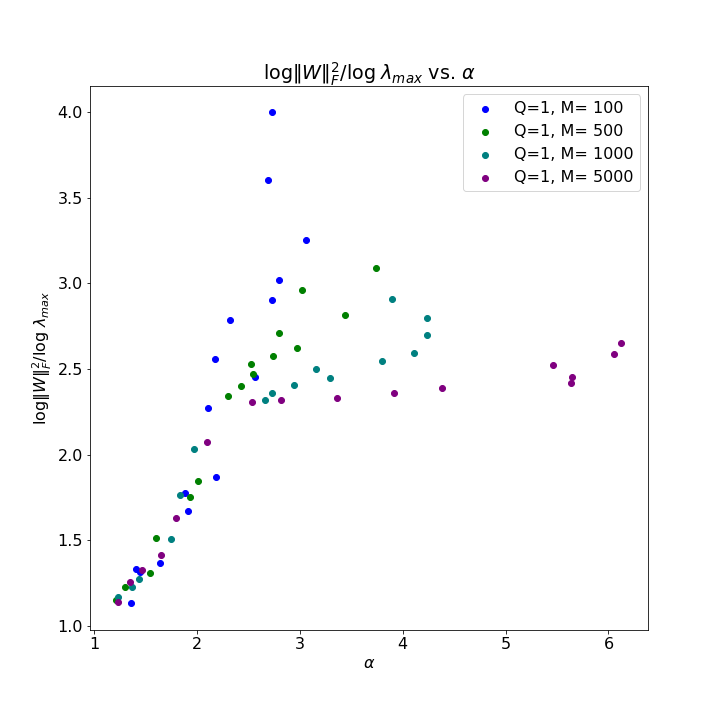
\includegraphics[scale=0.40]{img/Alpha-LogNorm-Relations.png}
   \caption{
Numerical test of the  Power Law - Norm Relation for random Heavy Tailed matrices
}
  \label{fig:randW}
\end{figure}

\charlesX{Describe here.

The numerical results for the the Power Law-Norm relation shows several interesting features: 

First, as $\alpha$ increases, the Log-units Stable Rank increases.  Then it

\begin{itemize}
\item
is very clear for $\alpha<2$ 
\item
saturates for $\alpha>2$  for large M
\item
extends beyond $\alpha>2$  because of finite size effects
\end{itemize}

}

\charlesX{I am not sure why the slope is not negative...the eigenvalues are VERY LARGE, and $\log\lambda_{max}~3-5$ so this just is OFF.
Are we missing something in the derivation, like the fact that the norm squared has to be positive ?  HELP}


\paragraph{Defining the Layer Weight Matrices}
\charles{Here we describe how we exact the matrices.  We have not done this yet for convolutional layers--thats \emph{another} paper}

$$\text{Linear Layer:}\;\;\log\Vert\mathbf{W}_{l}\Vert^{2}\rightarrow b_{l}\alpha_{l}$$

For the Conv2D layers, we relate the 'Norm' of the 4-index Tensor $\mathbf{W}_{l}$ to the sum of the integrals of the $n=c\times d$ ESDs for each feature map, giving 

$$\text{Conv2D Layer:}\;\;\log\Vert\mathbf{W}_{l}\Vert^{2}\rightarrow \sum_{i}b_{i,l}\alpha_{i,l}$$

So in the expression for the product norm for $\log\mathcal{C}$, let us replace each $\log\Vert\mathbf{W}_{l}\Vert$ for layer $l$ with the sum of the power law exponents $\alpha_{l,i}$ for the $n{_l}$ $\mathbf{W}_{l,i}$ layer matrices, and take the average over all $N_{\alpha}$  matrices.  This lets us relate the product norm complexity metric to the weighted average of power law exponents

where

$$\hat{\alpha}:=\dfrac{1}{N_{\alpha}}\sum_{i,l}b_{i,j}\alpha_{i,l}$$


We can now use $\hat{\alpha}$ ,  or, equivalently, $2\langle\log\Vert\mathbf{W}\Vert\rangle$ to analyze numerous pre-trained DNNs...and the results are indeed surprising.

I HAVE PLOTS FOR BOTH !
Which should we display ?  


\michael{How to resolve normalization issue ?

We need a normalizer $K$ that 

$$K\int_{0}^{\lambda_{max}}\rho(\lambda)d\lambda=1$$

and we know that our final expression is off by a sign in alpha

So we need a normalizer that has

 $$K\sim\lambda^{2\alpha}_{max}$$
 
 or maybe 
 
  $$K\sim\lambda^{2\alpha-2}_{max}$$

But also know that 
 
 $$\int_{0}^{\lambda_{max}}\rho(\lambda)d\lambda=\dfrac{1}{1-\alpha}\lambda_{max}^{1-\alpha}$$
which suggests that

$$K\dfrac{1}{1-\alpha}\lambda_{max}^{1-\alpha}=1$$

and that we might write K 
$$K=(\alpha-1)\lambda_{max}^{1-\alpha}$$

notice we use $(\alpha-1)$ and not $(1-\alpha)$ since $\alpha>1$...but I think we need something like

$$K[\dfrac{1}{1-\alpha}\lambda_{max}^{1-\alpha}]^{2}=1$$

giving

$$K=(1-\alpha)^{2}\lambda_{max}^{2\alpha-2}$$

But this gives the wrong expression for the integral

$$K\int_{0}^{\lambda_{max}}\rho(\lambda)d\lambda=1$$

and only works for

$$K[\int_{0}^{\lambda_{max}}\rho(\lambda)d\lambda]^{2}=1$$

and I don't know how to stick it back into the formula for the Trace to get right result
}
\charles{
I actually think most of this is wrong and that we need to be more clever
For example, see
http://www-personal.umich.edu/~mejn/courses/2006/cmplxsys899/powerlaws.pdf

where they derive  an expression for the expected max eigenvalue $\langle\lambda_{max}\rangle$
in terns of M, for an non-truncated power law

$$\langle\lambda_{max}\rangle\sim M^{1/(\alpha-1)}$$

So we would have  ($\alpha>1$)

$$\log\langle\lambda_{max}\rangle\sim\dfrac{1}{\alpha-1}\log\;M$$

or
$$(\alpha-1)\log\langle\lambda_{max}\rangle\sim\log\;M$$

Now maybe in our case there is some way to add in information about the norm of W
on the R.H.S. where the log M term arises   ?

}

